%! Licence = CC BY-NC-SA 4.0

%! Author = mariuszindel
%! Date = 06. Jul 2021
%! Project = DS1-Summary

\section{Introduction}


\subsection{Definition}
\textbf{English:} A distributed system in its simplest definition is a group of computers working together as to appear as a single computer to the user.\\
\textbf{German:} Ein verteiltes System in seiner einfachsten Definition ist eine Gruppe von Computern, die so zusammenarbeiten, dass sie dem Benutzer als ein einziger Computer erscheinen.

\subsection{Motivation}

\subsubsection{Scaling}
\paragraph{Vertical}
\textbf{Moore's Law: }Nr. of transistors doubles every 2 years.\\
\textbf{Nielsen's Law:} High-end user's connection speed grows by 50\% per year.\\
\textit{$\rightarrow$ Bandwidth grows slower than computer power!}\\
\textbf{Kryder's Law:} Disk density doubling every 13 month.
\begin{itemize}[label={\textcolor{ForestGreen}{+}}]
    \item Lower cost with small scale
    \item No adaption of software required
    \item Less administrative effort
\end{itemize}
\begin{itemize}[label={\textcolor{red}{--}}]
    \item HW limits for scaling
    \item Risk of HW failure causing outage
    \item More difficult to add fault tolerance
\end{itemize}
\paragraph{Horizontal}
\begin{itemize}[label={\textcolor{ForestGreen}{+}}]
    \item Lower cost with massive scale
    \item Easier to add fault-tolerance
    \item Higher availability
\end{itemize}
\begin{itemize}[label={\textcolor{red}{--}}]
    \item Adaption of software required
    \item More complex system, more components involved
\end{itemize}

\subsubsection{Economics}
\begin{minipage}{0.6\linewidth}
    \begin{itemize}
        \item Initially scaling vertically is cheaper, until you max out hardware.
        \item Current x86 max: 64 cores / 128 threads
    \end{itemize}
\end{minipage}
\begin{minipage}{0.45\linewidth}
\begin{center}
    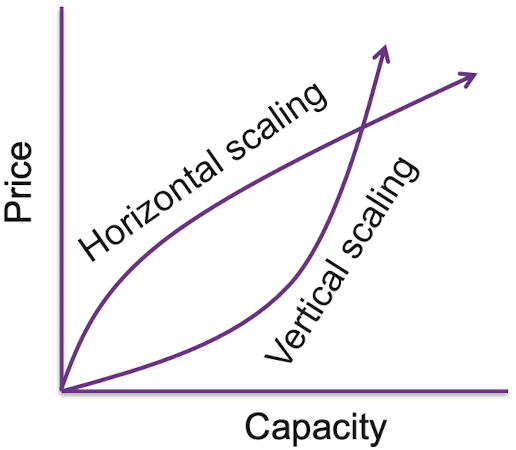
\includegraphics[scale=.25]{01-Introduction/Economics.png}    
\end{center}
\end{minipage}


\subsubsection{Location}
\begin{itemize}
    \item Everything gets faster, latency stays
    \item Physically bounded by the speed of light
    \item New protocols can decrease round trip
    \item Place services closer to user
\end{itemize}

\subsubsection{Fault Tolerance}
\begin{itemize}
    \item Any hardware will crash eventually
    \item Random bit flips in memory
    \item Error-correcting code memory (ECC RAM)
    \begin{itemize}
        \item Uses TMR or Hamming Code
        \item correct 1 bitflip / detect 2 bitflips 
        \item Used for Servers / MAC Pro 2020
    \end{itemize}
\end{itemize}


\subsection{Categorization}
\subsubsection{Kind of Distributed Systems:}
\paragraph{Coupling}
\begin{itemize}
    \item Tightly Coupled $\rightarrow$ Processing Elements have access to a common memory
    \item Loosely Coupled $\rightarrow$ Processing Elements have  no access to a common memory
\end{itemize}
\paragraph{Processor:}
\begin{itemize}    
    \item homogeneous system $\rightarrow$ All processors are of the same type
    \item heterogeneous system $\rightarrow$ Processors of different types
\end{itemize}
\paragraph{Scaling:}
\begin{itemize}
    \item small-scale $\rightarrow$ WebApp + database
    \item large-scale$\rightarrow$ more than 2 machines
\end{itemize}


\subsubsection{"Controlled" Distributed Systems}
\paragraph{Properties:}
\begin{itemize}
    \item 1 responsible organization
    \item Low churn
    \item Secure environment
    \item High availability
    \item Homogenous / Heterogeneous
\end{itemize}
\paragraph{Example:}
Amazon DynamoDB, Client/Server architecture
\paragraph{Work well:} 
\begin{itemize}
    \item Consistent hashing (DynamoDB, Cassandra)
    \item Master nodes, central coordinator
    \item Network is under control or client/server
    \item No NAT issues
\end{itemize}
\paragraph{Consistency}
\begin{itemize}
    \item Leader election
\end{itemize}
\paragraph{Replication principles}
\begin{itemize}
    \item More replicas: higher availability / reliability / performance / scalability
    \item Requires maintaining consistency in replicas
\end{itemize}

\subsubsection{"Fully" Decentralized Systems}
\paragraph{Properties:}
\begin{itemize}
    \item N responsible organizations
    \item High churn
    \item Hostile environment
    \item Unpredictable availability
    \item Heterogeneous
\end{itemize}
\paragraph{Example:}
BitTorrent, Blockchain
\paragraph{Work well:} 
\begin{itemize}
    \item Consistent hashing (DHTs)
    \item Flooding/broadcasting (Bitcoin)
\end{itemize}
\paragraph{Problems:} 
\begin{itemize}
    \item NAT and direct connectivity huge problem
\end{itemize}
\paragraph{Consistency}
\begin{itemize}
    \item Weak consistency: DHTs
    \item Nakamoto consensus (aka proof of work)
    \item Proof of stake – Leader election
\end{itemize}
\paragraph{Replication principles}
\begin{itemize}
    \item apply to fully
\end{itemize}

\subsubsection{CAP theorem}
A distributed data store cannot simultaneously be consistent, available and partition tolerant!
\begin{itemize}
    \item \textbf{Consistency (Konsistenz)} Every node has the same consistent state
    \item \textbf{Availability (Verfügbarkeit)} Every non-failing node always returns a response
    \item \textbf{Partition Tolerant (Teilungstolerant)} The system continues to be consistent even when network partitions
\end{itemize}

\subsection{Transparency}
Distributed system should hide it's distributed nature
\begin{itemize}
    \item \textbf{Location:} users should not be aware of the physical location
    \item \textbf{Access:} users should access resources in a single, uniform way
    \item \textbf{Migration, relocation:} users should not be aware, that resources have moved
    \item \textbf{Replication:} Users should not be aware about replicas, it should appear as a single resource
    \item \textbf{Concurrency:} users should not be aware of other users
    \item \textbf{Failure:} Users should be aware of recovery mechanisms
    \item \textbf{Security:} Users should be minimally aware of security mechanisms
\end{itemize}

\subsection{Fallacies (Irrtümer)}
\begin{enumerate}
    \item The network is reliable
    \begin{itemize}
        \item Submarine cables
    \end{itemize}
    \item Latency is zero
    \begin{itemize}
        \item Ping to Australia is 300ms 
    \end{itemize}
    \item Bandwidth is infinite
    \begin{itemize}
        \item I.e. AWS Truck is faster than "the internet"
    \end{itemize}
    \item The network is secure
    \begin{itemize}
        \item Assume someone is listening. Don’t send sensitive data over the network.
    \end{itemize}
    \item Topology doesn’t change
    \begin{itemize}
        \item request can take different route than reply
    \end{itemize}
    \item There is one administrator
    \begin{itemize}
        \item route goes from one company to another rival company (UPC, Swisscom, ...)
    \end{itemize}
    \item Transport cost is zero
    \begin{itemize}
        \item Someone build and maintains the network
    \end{itemize}
    \item The network is homogenous
    \begin{itemize}
        \item fiber, WiFi copper / server, desktop, mobile
    \end{itemize}
\end{enumerate}

\vfill
$ $
\columnbreak
